% Flagship topic-relevance method: Policy Summary vs Firm-level Summary (T3/TEMP).
% Topic side: T3.5.2 (statements), T3.5.5 (yearly summaries, policy summary), T3.5.7 (embedding).
% Firm side:  T3.7.2 (yearly summaries of Item 1), T3.7.4 (firm-level summary), T3.7.6 (embedding).
% Score:      T3.8.2 (cosine of the two embeddings), measure "summaries | policy_summary | firm_summary".
% Compile:    pdflatex fig_topic_relevance_flagship_flowchart.tex
\documentclass[border=8pt]{standalone}
\usepackage[T1]{fontenc}
\usepackage{tgtermes}
\usepackage{tikz}
\usetikzlibrary{positioning, shapes.symbols, shadows, arrows.meta, fit, backgrounds, calc}

% Figure Style Guide colors (S3)
\definecolor{RED}{HTML}{B31942}
\definecolor{BLUE}{HTML}{0A3161}
\definecolor{MIDNIGHTBLUE}{HTML}{004953}
\definecolor{GREY}{HTML}{A6A6A8}
\definecolor{BLACK}{HTML}{101820}
\colorlet{SUBTEXT}{GREY!35!BLACK}

% second line inside a block: the fact behind the block, in small dark grey
\newcommand{\sub}[1]{\\[2pt]{\scriptsize\color{SUBTEXT}#1}}

\begin{document}
\hyphenpenalty=10000 \exhyphenpenalty=10000
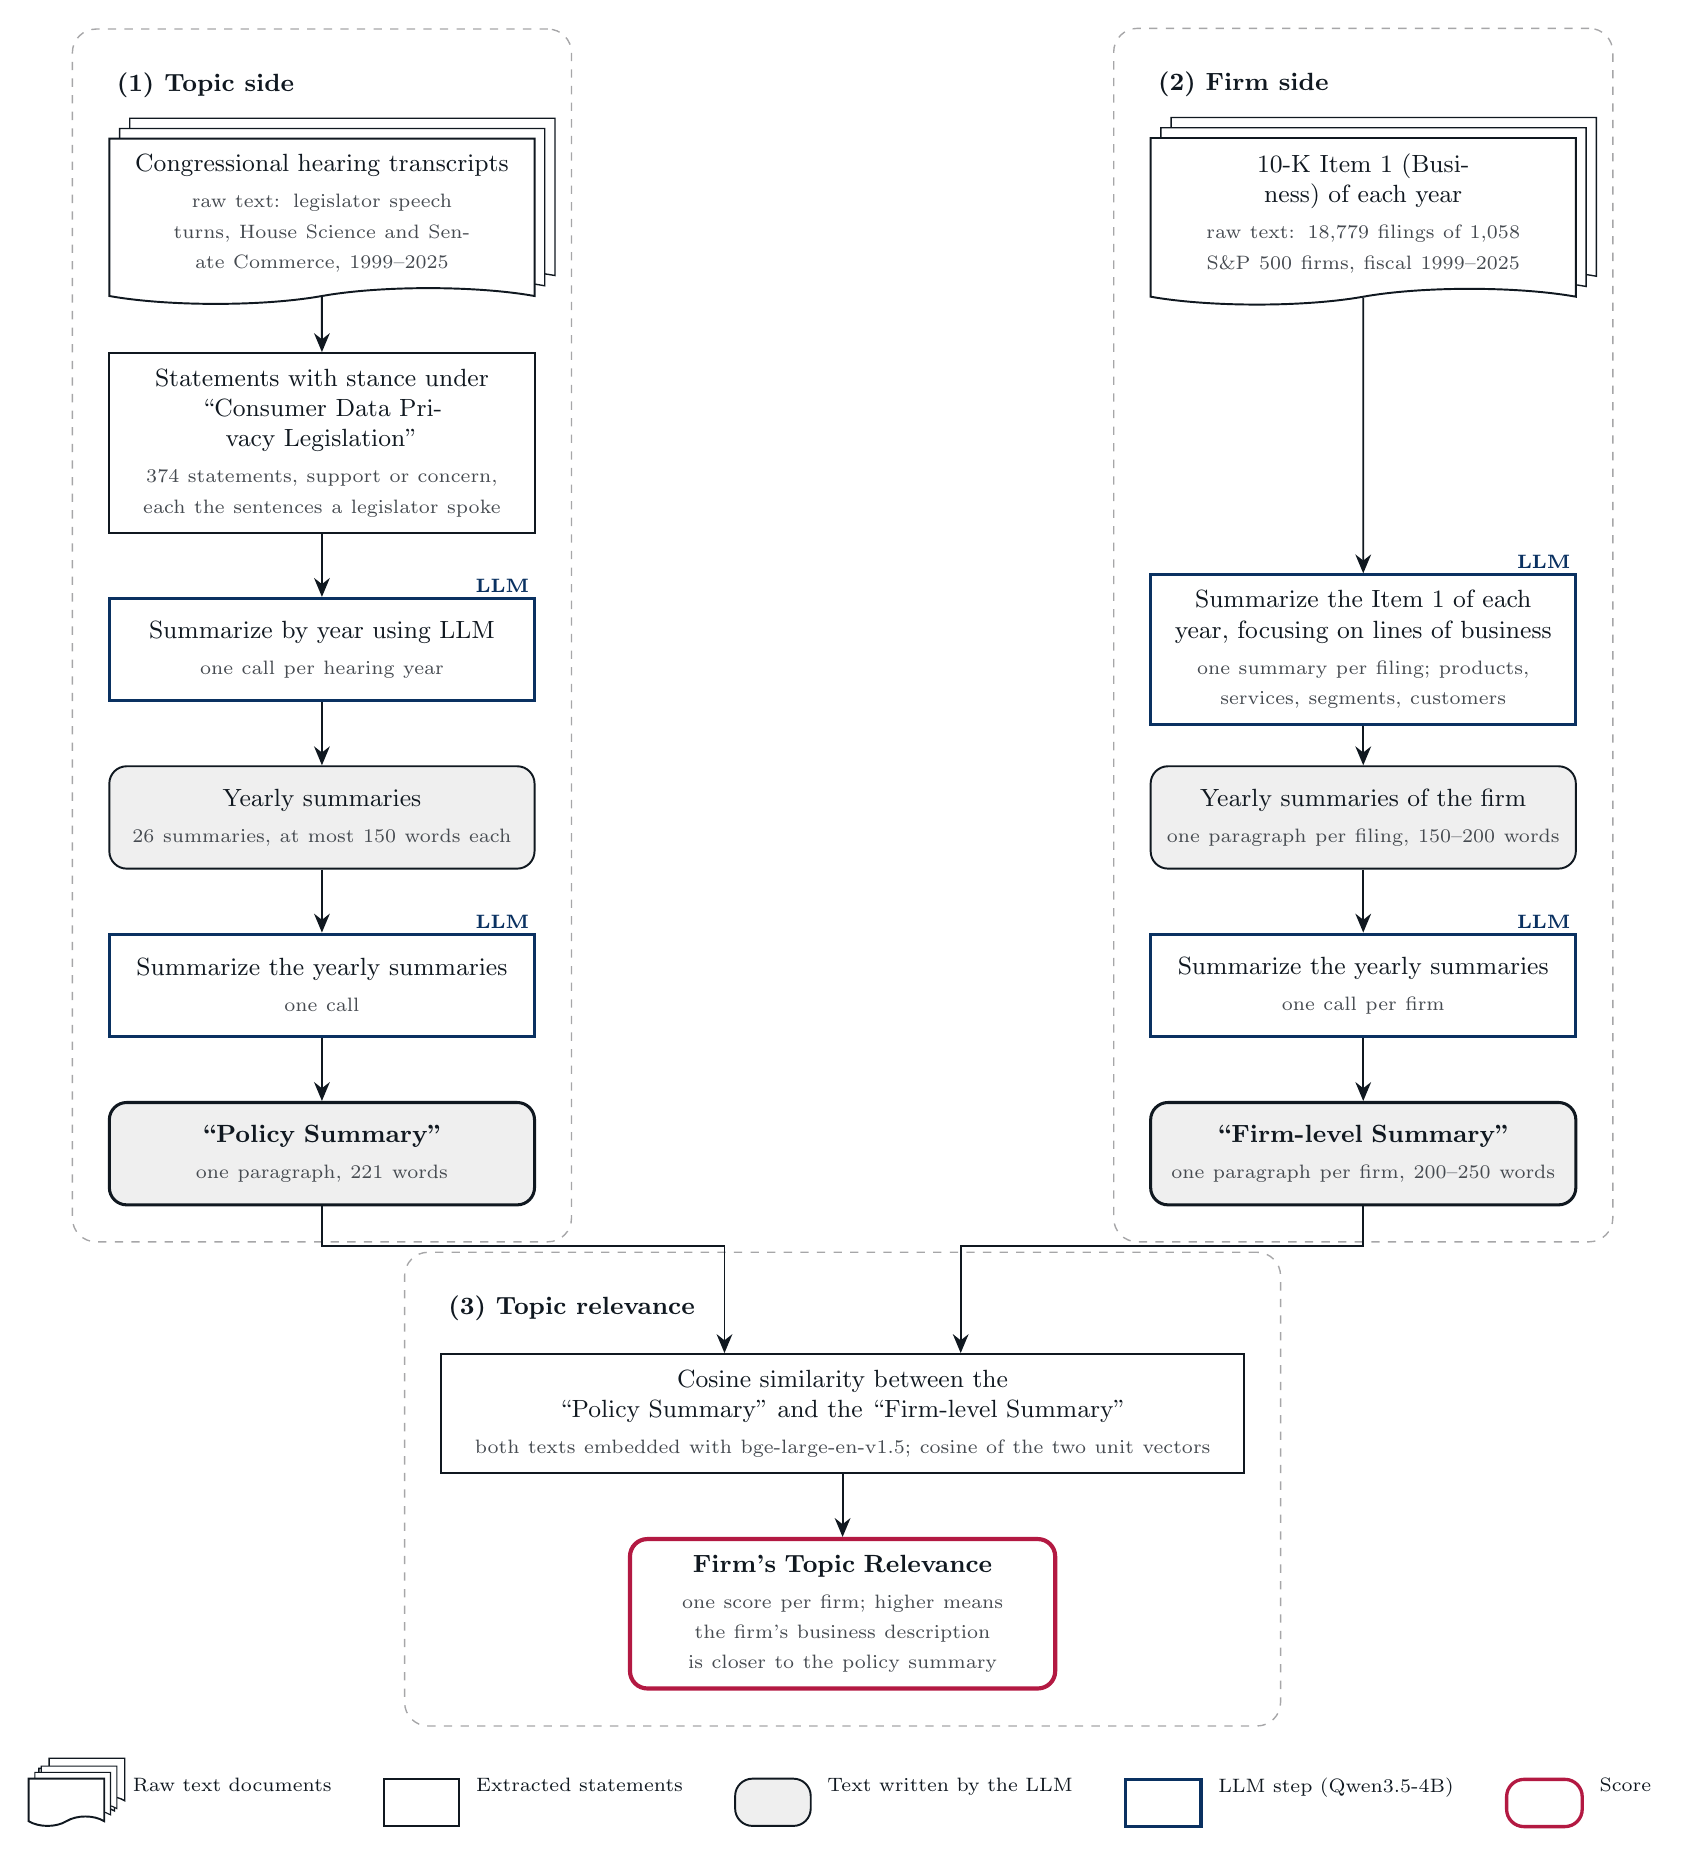
\begin{tikzpicture}[
  font=\small, text=BLACK, color=BLACK,
  node distance=8mm and 14mm,
  every node/.style={align=center},
  flow/.style={-{Stealth[length=2.4mm, width=2mm]}, line width=0.7pt, BLACK},
  % raw text: a stack of documents with a torn lower edge
  rawdoc/.style={tape, tape bend top=none, tape bend height=2mm, draw=BLACK, line width=0.7pt, fill=white,
                 text width=50mm, minimum height=15mm, inner sep=2mm,
                 double copy shadow={shadow xshift=1.3mm, shadow yshift=1.3mm, draw=BLACK, fill=white, line width=0.5pt}},
  % extracted statements: lines of text with a bar at the left, as quoted sentences
  statements/.style={rectangle, draw=BLACK, line width=0.7pt, fill=white, text width=50mm, minimum height=15mm, inner sep=2mm,
                 append after command={\pgfextra{\draw[BLACK, line width=2.4pt]
                   ($(\tikzlastnode.north west)+(1.3mm,-1.3mm)$) -- ($(\tikzlastnode.south west)+(1.3mm,1.3mm)$);}}},
  % text written by the LLM: rounded, shaded
  summary/.style={rectangle, rounded corners=2.2mm, draw=BLACK, line width=0.7pt, fill=GREY!18,
                  text width=50mm, minimum height=13mm, inner sep=2mm},
  % LLM step: process box in BLUE with an LLM tag
  llm/.style={rectangle, draw=BLUE, line width=1.1pt, fill=white, text width=50mm, minimum height=13mm, inner sep=2mm,
              label={[text=BLUE, font=\scriptsize\bfseries, anchor=south east, inner sep=0pt, xshift=-0.8mm, yshift=0.5mm]north east:LLM}},
  % calculation step and the final score
  calcstep/.style={rectangle, draw=BLACK, line width=0.7pt, fill=white, text width=98mm, minimum height=13mm, inner sep=2mm},
  output/.style={rectangle, rounded corners=2.2mm, draw=RED, line width=1.5pt, fill=white, text width=50mm, minimum height=13mm, inner sep=2mm},
  lane/.style={draw=GREY, line width=0.5pt, dashed, rounded corners=3mm, inner sep=4.5mm},
  lanetitle/.style={font=\small\bfseries, text=BLACK, anchor=south west, inner sep=1mm},
]

% ---------------------------------------------------------------- (1) Topic side
\node[rawdoc] (T1) {Congressional hearing transcripts\sub{raw text: legislator speech turns, House Science and Senate Commerce, 1999--2025}};
\node[statements, below=of T1] (T2) {Statements with stance under\\ ``Consumer Data Privacy Legislation''\sub{374 statements, support or concern, each the sentences a legislator spoke}};
\node[llm, below=of T2] (T3) {Summarize by year using LLM\sub{one call per hearing year}};
\node[summary, below=of T3] (T4) {Yearly summaries\sub{26 summaries, at most 150 words each}};
\node[llm, below=of T4] (T5) {Summarize the yearly summaries\sub{one call}};
\node[summary, below=of T5, line width=1.1pt] (T6) {\textbf{``Policy Summary''}\sub{one paragraph, 221 words}};

% ---------------------------------------------------------------- (2) Firm side
\node[rawdoc, right=78mm of T1] (F1) {10-K Item 1 (Business) of each year\sub{raw text: 18,779 filings of 1,058 S\&P 500 firms, fiscal 1999--2025}};
\node[llm] (F3) at (T3 -| F1) {Summarize the Item 1 of each year, focusing on lines of business\sub{one summary per filing; products, services, segments, customers}};
\node[summary] (F4) at (T4 -| F1) {Yearly summaries of the firm\sub{one paragraph per filing, 150--200 words}};
\node[llm] (F5) at (T5 -| F1) {Summarize the yearly summaries\sub{one call per firm}};
\node[summary, line width=1.1pt] (F6) at (T6 -| F1) {\textbf{``Firm-level Summary''}\sub{one paragraph per firm, 200--250 words}};

% ---------------------------------------------------------------- (3) Topic relevance
\node[calcstep] (C1) at ($(T6)!0.5!(F6)+(0,-33mm)$) {Cosine similarity between the\\ ``Policy Summary'' and the ``Firm-level Summary''\sub{both texts embedded with bge-large-en-v1.5; cosine of the two unit vectors}};
\node[output, below=of C1] (C2) {\textbf{Firm's Topic Relevance}\sub{one score per firm; higher means the firm's business description is closer to the policy summary}};

% ---------------------------------------------------------------- flows
\draw[flow] (T1) -- (T2);
\draw[flow] (T2) -- (T3);
\draw[flow] (T3) -- (T4);
\draw[flow] (T4) -- (T5);
\draw[flow] (T5) -- (T6);
\draw[flow] (F1) -- (F3);
\draw[flow] (F3) -- (F4);
\draw[flow] (F4) -- (F5);
\draw[flow] (F5) -- (F6);
\draw[flow] (T6.south) -- ++(0,-5mm) -| ([xshift=-15mm]C1.north);
\draw[flow] (F6.south) -- ++(0,-5mm) -| ([xshift=15mm]C1.north);
\draw[flow] (C1) -- (C2);

% ---------------------------------------------------------------- lanes and titles
\node[lanetitle] (titleT) at ([yshift=4mm]T1.north west) {(1) Topic side};
\node[lanetitle] (titleF) at ([yshift=4mm]F1.north west) {(2) Firm side};
\node[lanetitle] (titleC) at ([yshift=3mm]C1.north west) {(3) Topic relevance};
\begin{scope}[on background layer]
  \node[lane, fit=(titleT)(T1)(T6)] {};
  \node[lane, fit=(titleF)(F1)(F6)] {};
  \node[lane, fit=(titleC)(C1)(C2)] {};
\end{scope}

% ---------------------------------------------------------------- legend
% One matrix node, anchored at the midpoint between the two lanes, so the legend is centered under them.
\matrix[anchor=north, inner sep=0pt, column sep=1.2mm, row sep=0pt, nodes={inner xsep=0.8mm}] (legend) at ($(C2.south -| C1)+(0,-11mm)$) {
  \node[rawdoc, text width=8mm, minimum height=6mm, inner sep=0.8mm, tape bend height=1.2mm,
        double copy shadow={shadow xshift=0.8mm, shadow yshift=0.8mm, draw=BLACK, fill=white, line width=0.4pt}] {}; &[1.5mm]
  \node[font=\scriptsize] {Raw text documents}; &[4.5mm]
  \node[statements, text width=8mm, minimum height=6mm, inner sep=0.8mm] {}; &
  \node[font=\scriptsize] {Extracted statements}; &[4.5mm]
  \node[summary, text width=8mm, minimum height=6mm, inner sep=0.8mm] {}; &
  \node[font=\scriptsize] {Text written by the LLM}; &[4.5mm]
  \node[rectangle, draw=BLUE, line width=1.1pt, fill=white, text width=8mm, minimum height=6mm, inner sep=0.8mm] {}; &
  \node[font=\scriptsize] {LLM step (Qwen3.5-4B)}; &[4.5mm]
  \node[output, text width=8mm, minimum height=6mm, inner sep=0.8mm, line width=1.2pt] {}; &
  \node[font=\scriptsize] {Score}; \\
};

\end{tikzpicture}
\end{document}
